\subsection{Feature Module: Generating View Descriptors}
\label{sec:architecture-feature-module}
The objective of the feature module is the generation of a descriptor for each view $v$ by using five convolutional layers.
Each one is referred to as a view descriptor $\vec{V}^{[l]}_v$ of the $l$-th layer in the following.
\figref{fig:feature-module} shows the basic concept.
\begin{figure}
	\centering
	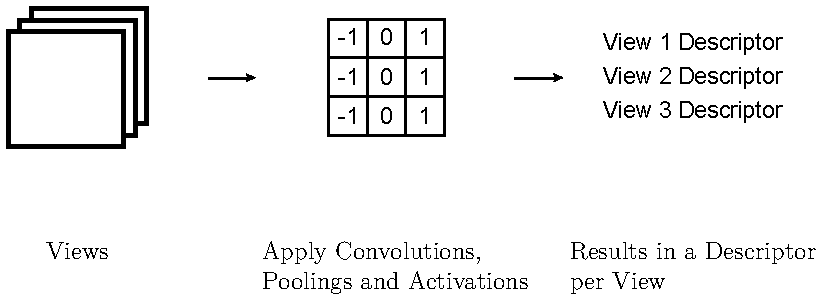
\includegraphics[]{images/feature_module.pdf}
	\caption{Basic concept of the feature module. On each view $v$ of a multi-view $\tilde{\vec{X}}^{(i)}$ of the $i$-th sample convolutions and poolings are performed yielding the final view descriptors $\vec{V}^{[5]}_v$.}
	\label{fig:feature-module}
\end{figure}
This module is the first one in the feed-forward chain.
Its input is a multi-view $\tilde{\vec{X}}^{(i)}$ of the $i$-th object.
Because tensorflow supports batch execution, i.\,e. all its operations can be applied to a batch of data, the multi-view input is converted to a tensor with a batch dimension for multiple multi-views.
This yields an input tensor of shape $Batch \times Views \times Height \times Width \times Channels$.
In the following, if a tensor has a batch dimension, which is usually the case, it is assumed that any mentioned operation or approach is applied to every batch element.
This module consists of five main convolutional layers.
A main convolutional layer consists of a convolutional layer and an optional pooling layer.
The first main layer performs a valid convolution with 96 filters $\vec{K}^{[1]}$ of size $7 \times 7$ and a stride of $s=2$ on each $224 \times 224 \times 3$ multi-view view.
Every filter extracts different features.
In comparison, the original AlexNet uses filters $\vec{K}^{[1]}$ of size $11 \times 11$ and a stride of $s=4$.
However, it is assumed that smaller filters and a smaller stride are collecting more information that can be used for a classification of the object and material at once.
A convolution operation is performed by moving a filter across a input and calculating each dot product.
This results in the view descriptor $\vec{V}^{[1]}$ with a size of $Views \times 109 \times 109 \times 96$ in this case.
Furthermore, to each convolution output, the corresponding bias is added.
This result is fed into a ReLU activation function.
Finally, the outputs are max-pooled with a window $\vec{K}_{\text{max}}$ of size $3 \times 3$ and a stride of $s=2$.
No padding is applied.
It is defined, that the max-pooling is always performed on the last dimension, i.\,e. the one containing each feature.
This yields a matrix of shape $Views \times 54 \times 54 \times 96$ for each pooling in the first main convolutional layer.
For simplicity, it is defined that within each main layer the view descriptor is reused.
Hence, the output of the $l$-th main layer is the view descriptor $\vec{V}^{[l]}$.
The next layers are similar including the bias addition and the ReLU activation function.
Hence, only the operations and their parameters will be mentioned.
Furthermore, the layers are added sequentially.
That means, the activations of the previous main layer are the input of the current main layer and so on.
The second main layer performs a convolution with 256 filters $\vec{K}^{[2]}$ of size $5 \times 5$ and a stride of $s=2$.
However, this time the input is padded in a way, that the output has the original input's size.
This yields a convolution result $\vec{V}^{[2]}$ of shape $Views \times 27 \times 27 \times 256$.
The max-pooling uses again a window $\vec{K}_{\text{max}}$ of $3 \times 3$ and a stride of $s=2$.
The valid padding technique is applied resulting in a shape of $Views \times 13 \times 13 \times 256$.
The third and fourth main layer use 384 filters $\vec{K}^{[3]}$ and $\vec{K}^{[4]}$ of size $3 \times 3$ for the convolution task with a stride of $s=1$ each and the padding technique same.
However, no pooling is performed.
Hence, this yields a matrix $\vec{V}^{[3]}$ and $\vec{V}^{[4]}$ of shape $Views \times 13 \times 13 \times 384$ both the times.
For the last main layer, the fifth one, a convolution with 256 filters $\vec{K}^{[5]}$ of size $3 \times 3$ is performed.
The stride is $s=1$ and the padding technique same, hence, the result $\vec{V}^{[5]}$ has a size of $Views \times 13 \times 13 \times 256$.
The output's dimension is reduced with a valid max-pooling $\vec{K}_{\text{max}}$ of size $3 \times 3$ and stride $s=2$ to $Views \times 6 \times 6 \times 256$.
In the end, this whole process results in a tensor $\bar{\vec{V}}^{[5]}$ containing each view's view descriptor $\vec{V}^{[5]}$ of size $Views \times 6 \times 6 \times 256$ of every batch element.
Hence, this tensor's shape is $Batch \times Views \times 6 \times 6 \times 256$.